\documentclass[a4paper]{scrartcl}
\usepackage{amssymb, amsmath} % needed for math
\usepackage{mathtools}      % \xRightarrow
\usepackage[utf8]{inputenc} % this is needed for umlauts
\usepackage[english]{babel} % this is needed for umlauts
\usepackage[T1]{fontenc}    % this is needed for correct output of umlauts in pdf
\usepackage[margin=2.5cm]{geometry} %layout
\usepackage{hyperref}   % links im text
\usepackage{braket}         % needed for \Set
\usepackage{parskip}
\usepackage[colorinlistoftodos]{todonotes}
\usepackage{pgfplots}
\pgfplotsset{compat=1.7,compat/path replacement=1.5.1}
\usepackage{tikz}

\title{Minimal distance to a cubic function}
\author{Martin Thoma}

\hypersetup{ 
  pdfauthor   = {Martin Thoma}, 
  pdfkeywords = {}, 
  pdftitle    = {Minimal Distance} 
}

\def\mdr{\ensuremath{\mathbb{R}}}

%%%%%%%%%%%%%%%%%%%%%%%%%%%%%%%%%%%%%%%%%%%%%%%%%%%%%%%%%%%%%%%%%%%%%
% Begin document                                                    %
%%%%%%%%%%%%%%%%%%%%%%%%%%%%%%%%%%%%%%%%%%%%%%%%%%%%%%%%%%%%%%%%%%%%%
\begin{document}
\maketitle
\begin{abstract}
When you have a selfdriving car, you have to plan which path you
want to take. A reasonable choice for the representation of this
path is a cubic spline. But you also have to be able to calculate
how to steer to get or to remain on this path. A way to do this
is applying the \href{https://en.wikipedia.org/wiki/PID_algorithm}{PID algorithm}.
But this algorithm needs to know the current error. So you need to 
be able to get the minimal distance of a point to a cubic spline.
As you need to get the signed error (and one steering direction might
be prefered), it is not only necessary to
get the minimal absolute distance, but also to get all points
on the spline with minimal distance.

In this paper I want to discuss how to find all points on a cubic 
function with minimal distance to a given point.
As other representations of paths might be easier to understand and
to implement, I will also cover the problem of finding the minimal
distance of a point to a polynomial of degree 0, 1 and 2.
\end{abstract}

\section{Description of the Problem}
Let $f: \mdr \rightarrow \mdr$ be a polynomial function and $P \in \mdr^2$
be a point. Let $d: \mdr^2 \times \mdr^2 \rightarrow \mdr_0^+$
be the Euklidean distance of two points:
\[d \left ((x_1, y_1), (x_2, y_2) \right) := \sqrt{(x_1 - x_2)^2 + (y_1 - y_2)^2}\]

Now there is \todo{Should I proof this?}{finite set} $x_1, \dots, x_n$ such that 
\[\forall \tilde x \in \mathbb{R} \setminus \{x_1, \dots, x_n\}: d(P, (x_1, f(x_1))) = \dots = d(P, (x_n, f(x_n))) < d(P, (\tilde x, f(\tilde x)))\]

The task is now to find those $x_1, \dots, x_n$ for given $f, P$.

\section{Minimal distance to a constant function}
Let $f(x) = c$ with $c \in \mdr$ be a constant function. 

\begin{figure}[htp]
    \centering
    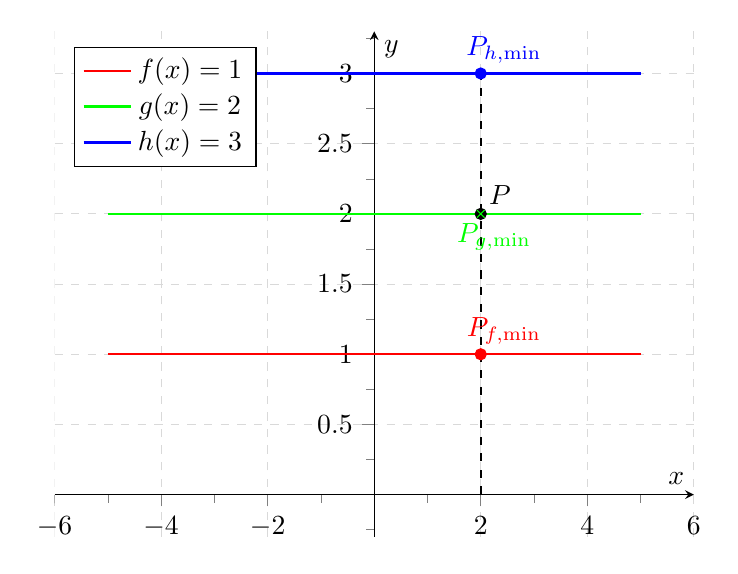
\begin{tikzpicture}
        \begin{axis}[
            legend pos=north west,
            axis x line=middle,
            axis y line=middle,
            grid = major,
            width=0.8\linewidth,
            height=8cm,
            grid style={dashed, gray!30},
            xmin=-5, % start the diagram at this x-coordinate
            xmax= 5, % end   the diagram at this x-coordinate
            ymin= 0, % start the diagram at this y-coordinate
            ymax= 3, % end   the diagram at this y-coordinate
            axis background/.style={fill=white},
            xlabel=$x$,
            ylabel=$y$,
            tick align=outside,
            minor tick num=-3,
            enlargelimits=true,
            tension=0.08]
          \addplot[domain=-5:5, thick,samples=50, red] {1};
          \addplot[domain=-5:5, thick,samples=50, green] {2};
          \addplot[domain=-5:5, thick,samples=50, blue] {3};
          \addplot[black, mark = *, nodes near coords=$P$,every node near coord/.style={anchor=225}] coordinates {(2, 2)};
          \addplot[blue, mark = *, nodes near coords=$P_{h,\text{min}}$,every node near coord/.style={anchor=225}] coordinates {(2, 3)};
          \addplot[green, mark = x, nodes near coords=$P_{g,\text{min}}$,every node near coord/.style={anchor=120}] coordinates {(2, 2)};
          \addplot[red, mark = *, nodes near coords=$P_{f,\text{min}}$,every node near coord/.style={anchor=225}] coordinates {(2, 1)};
          \draw[thick, dashed] (axis cs:2,0) -- (axis cs:2,3);
          \addlegendentry{$f(x)=1$}
          \addlegendentry{$g(x)=2$}
          \addlegendentry{$h(x)=3$}
        \end{axis} 
    \end{tikzpicture}
    \caption{3 constant functions and their points with minimal distance}
    \label{fig:constant-min-distance}
\end{figure}

Then $(x_P,f(x_P))$ has
minimal distance to $P$. Every other point has higher distance.
See Figure~\ref{fig:constant-min-distance}.

\section{Minimal distance to a linear function}
Let $f(x) = m \cdot x + t$ with $m \in \mdr \setminus \Set{0}$ and 
$t \in \mdr$ be a linear function.

\begin{figure}[htp]
    \centering
    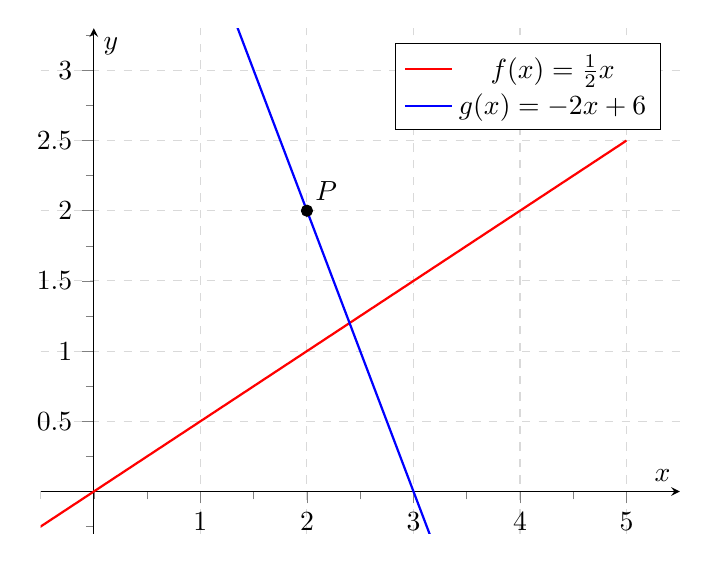
\begin{tikzpicture}
        \begin{axis}[
            legend pos=north east,
            axis x line=middle,
            axis y line=middle,
            grid = major,
            width=0.8\linewidth,
            height=8cm,
            grid style={dashed, gray!30},
            xmin= 0, % start the diagram at this x-coordinate
            xmax= 5, % end   the diagram at this x-coordinate
            ymin= 0, % start the diagram at this y-coordinate
            ymax= 3, % end   the diagram at this y-coordinate
            axis background/.style={fill=white},
            xlabel=$x$,
            ylabel=$y$,
            tick align=outside,
            minor tick num=-3,
            enlargelimits=true,
            tension=0.08]
          \addplot[domain=-5:5, thick,samples=50, red] {0.5*x};
          \addplot[domain=-5:5, thick,samples=50, blue] {-2*x+6};
          \addplot[black, mark = *, nodes near coords=$P$,every node near coord/.style={anchor=225}] coordinates {(2, 2)};
          \addlegendentry{$f(x)=\frac{1}{2}x$}
          \addlegendentry{$g(x)=-2x+6$}
        \end{axis} 
    \end{tikzpicture}
    \caption{The shortest distance of $P$ to $f$ can be calculated by using the perpendicular}
    \label{fig:linear-min-distance}
\end{figure}

Now you can drop a perpendicular $f_\bot$ through $P$ on $f(x)$. The slope of $f_\bot$
is $- \frac{1}{m}$. Now you can calculate $f_\bot$:\nobreak
\begin{align}
                 f_\bot(x) &= - \frac{1}{m} \cdot x + t_\bot\\
    \Rightarrow        y_P &= - \frac{1}{m} \cdot x_P + t_\bot\\
    \Leftrightarrow t_\bot &= y_P + \frac{1}{m} \cdot x_P
\end{align}

Now find the point $(x, f(x))$ where the perpendicular crosses the function:
\begin{align}
    f(x) &= f_\bot(x)\\
    \Leftrightarrow m \cdot x + t &= - \frac{1}{m} \cdot x + \left(y_P + \frac{1}{m} \cdot x_P \right)\\
    \Leftrightarrow \left (m + \frac{1}{m} \right ) \cdot x &= y_P + \frac{1}{m} \cdot x_P - t\\
    \Leftrightarrow x &= \frac{m}{m^2+1} \left ( y_P + \frac{1}{m} \cdot x_P - t \right )
\end{align}

There is only one point with minimal distance. See Figure~\ref{fig:linear-min-distance}.
\clearpage
%%%%%%%%%%%%%%%%%%%%%%%%%%%%%%%%%%%%%%%%%%%%%%%%%%%%%%%%%%%%%%%%%%%%%
% Quadratic functions                                               %
%%%%%%%%%%%%%%%%%%%%%%%%%%%%%%%%%%%%%%%%%%%%%%%%%%%%%%%%%%%%%%%%%%%%%
\section{Minimal distance to a quadratic function}
Let $f(x) = a \cdot x^2 + b \cdot x + c$ with $a \in \mdr \setminus \Set{0}$ and 
$b, c \in \mdr$ be a quadratic function.

\begin{figure}[htp]
    \centering
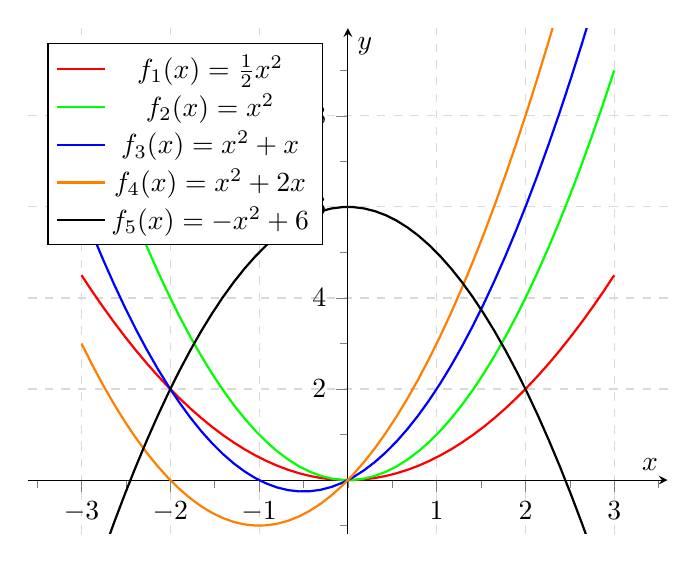
\begin{tikzpicture}
    \begin{axis}[
        legend pos=north west,
        axis x line=middle,
        axis y line=middle,
        grid = major,
        width=0.8\linewidth,
        height=8cm,
        grid style={dashed, gray!30},
        xmin=-3,     % start the diagram at this x-coordinate
        xmax= 3,    % end   the diagram at this x-coordinate
        ymin=-0.25,     % start the diagram at this y-coordinate
        ymax= 9,   % end   the diagram at this y-coordinate
        axis background/.style={fill=white},
        xlabel=$x$,
        ylabel=$y$,
        %xticklabels={-2,-1.6,...,7},
        %yticklabels={-8,-7,...,8},
        tick align=outside,
        minor tick num=-3,
        enlargelimits=true,
        tension=0.08]
      \addplot[domain=-3:3, thick,samples=50, red] {0.5*x*x}; 
      \addplot[domain=-3:3, thick,samples=50, green] {x*x}; 
      \addplot[domain=-3:3, thick,samples=50, blue] {x*x + x};
      \addplot[domain=-3:3, thick,samples=50, orange] {x*x + 2*x};
      \addplot[domain=-3:3, thick,samples=50, black] {-x*x + 6};
      \addlegendentry{$f_1(x)=\frac{1}{2}x^2$}
      \addlegendentry{$f_2(x)=x^2$}
      \addlegendentry{$f_3(x)=x^2+x$}
      \addlegendentry{$f_4(x)=x^2+2x$}
      \addlegendentry{$f_5(x)=-x^2+6$}
    \end{axis} 
\end{tikzpicture}
    \caption{Quadratic functions}
\end{figure}

\subsection{Number of points with minimal distance}
It is obvious that a quadratic function can have two points with 
minimal distance. 

For example, let $f(x) = x^2$ and $P = (0,5)$. Then $P_{f,1} \approx (2.179, 2.179^2)$
has minimal distance to $P$, but also $P_{f,2}\approx (-2.179, 2.179^2)$.

Obviously, there cannot be more than three points with minimal distance.
But can there be three points?

\begin{figure}[htp]
    \centering
    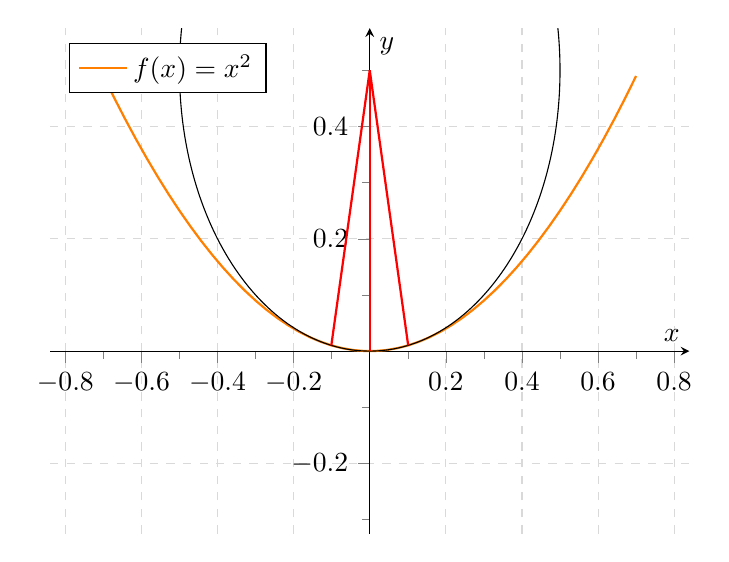
\begin{tikzpicture}
        \begin{axis}[
            legend pos=north west,
            axis x line=middle,
            axis y line=middle,
            grid = major,
            width=0.8\linewidth,
            height=8cm,
            grid style={dashed, gray!30},
            xmin=-0.7,     % start the diagram at this x-coordinate
            xmax= 0.7,    % end   the diagram at this x-coordinate
            ymin=-0.25,     % start the diagram at this y-coordinate
            ymax= 0.5,   % end   the diagram at this y-coordinate
            axis background/.style={fill=white},
            xlabel=$x$,
            ylabel=$y$,
            %xticklabels={-2,-1.6,...,7},
            %yticklabels={-8,-7,...,8},
            tick align=outside,
            minor tick num=-3,
            enlargelimits=true,
            tension=0.08]
          \addplot[domain=-0.7:0.7, thick,samples=50, orange] {x*x};
          \draw (axis cs:0,0.5) circle[radius=0.5];
          \draw[red, thick] (axis cs:0,0.5) -- (axis cs:0.101,0.0102);
          \draw[red, thick] (axis cs:0,0.5) -- (axis cs:-0.101,0.0102);
          \draw[red, thick] (axis cs:0,0.5) -- (axis cs:0,0);
          \addlegendentry{$f(x)=x^2$}
        \end{axis} 
    \end{tikzpicture}
    \caption{3 points with minimal distance?}
    \todo[inline]{Is this possible? http://math.stackexchange.com/q/553097/6876}
\end{figure}

As the point is already given, you want to minimize the following 
function:

\begin{align}
    d:   &\mdr \rightarrow \mdr^+_0\\
    d(x) &= \sqrt{(x_p,y_p),(x,f(x))}\\
         &= \sqrt{(x_p-x)^2 + (y_p - f(x))^2}\\
         &= \sqrt{x_p^2 - 2x_p x + x^2 + y_p^2 - 2y_p f(x) + f(x)^2}
\end{align}

Minimizing $d$ is the same as minimizing $d^2$:
\begin{align}
    d(x)^2    &= x_p^2 - 2x_p x + x^2 + y_p^2 - 2y_p f(x) + f(x)^2\\
    (d(x)^2)' &= -2 x_p + 2x -2y_p(f(x))' + (f(x)^2)'\\
           0  &\stackrel{!}{=} -2 x_p + 2x -2y_p(f(x))' + (f(x)^2)' \label{eq:minimizing}
\end{align}

Now we use thet $f(x) = ax^2 + bx + c$:

\begin{align}
    0     &\stackrel{!}{=} -2 x_p + 2x -2y_p(2ax+b) + ((ax^2+bx+c)^2)'\\
          &= -2 x_p + 2x -2y_p \cdot 2ax-2 y_p b + (a^2 x^4+2 a b x^3+2 a c x^2+b^2 x^2+2 b c x+c^2)'\\
          &= -2 x_p + 2x -4y_p ax-2 y_p b + (4a^2 x^3 + 6 ab x^2 + 4acx + 2b^2 x + 2bc)\\
          &= 4a^2 x^3 + 6 ab x^2 + 2(1 -2y_p a+ 2ac + b^2)x +2(bc-by_p-x_p)\\
\end{align}

\subsubsection{Solutions}
As the problem stated above is a cubic equation, you can solved it
analytically. But the solutions are not very nice, so I've entered

\texttt{$0=4*a^2 *x^3 + 6 *a*b *x^2 + 2*(1 -2*e *a+ 2*a*c + b^2)*x +2*(b*c-b*e-d)$}

with $d := x_p$ and $e := y_p$.

to \href{http://www.wolframalpha.com/input/?i=0%3D4*a%5E2+*x%5E3+%2B+6+*a*b+*x%5E2+%2B+2*%281+-2*e+*a%2B+2*a*c+%2B+b%5E2%29*x+%2B2*%28b*c-b*e-d%29}{WolframAlpha} to let it solve. The solutions are:

\textbf{First solution}

\begin{align*}
    x = &\frac{1}{6 \sqrt[3]{2} a^2} \sqrt[3]{(108 a^4 d+54 a^3 b+\sqrt{(108 a^4 d+54 a^3 b)^2+4 (12 a^3 c-12 a^3 e-3 a^2 b^2+6 a^2)^3})}\\
        &-\frac{12 a^3 c-12 a^3 e-3 a^2 b^2+6 a^2}
         {3 (2^{\frac{2}{3}}) a^2 \sqrt[3]{108 a^4 d+54 a^3 b+\sqrt{(108 a^4 d+54 a^3 b)^2+4 (12 a^3 c-12 a^3 e-3 a^2 b^2+6 a^2)^3}} }-b/(2 a)
\end{align*}

So the minimum for $a=1, b=c=d=0$ is:


\subsection{Calculate points with minimal distance}
\todo[inline]{Write this}
%%%%%%%%%%%%%%%%%%%%%%%%%%%%%%%%%%%%%%%%%%%%%%%%%%%%%%%%%%%%%%%%%%%%%
% Cubic                                                             %
%%%%%%%%%%%%%%%%%%%%%%%%%%%%%%%%%%%%%%%%%%%%%%%%%%%%%%%%%%%%%%%%%%%%%
\section{Minimal distance to a cubic function}
Let $f(x) = a \cdot x^3 + b \cdot x^2 + c \cdot x + d$ be a cubic function
with $a \in \mdr \setminus \Set{0}$ and 
$b, c, d \in \mdr$ be a function.

\subsection{Number of points with minimal distance}

\todo[inline]{Write this}

\subsection{Special points}
\todo[inline]{Write this}

\subsection{Voronoi}

For $b^2 \geq 3ac$

\todo[inline]{Write this}
\subsection{Calculate points with minimal distance}
When you want to calculate points with minimal distance, you can 
take the same approach as in Equation \ref{eq:minimizing}:

\begin{align}
    0  &\stackrel{!}{=} -2 x_p + 2x -2y_p(f(x))' + (f(x)^2)'\\
    \Leftrightarrow 0 &\stackrel{!}{=} 2 f(x) \cdot f'(x) - 2 y_p f'(x) + 2x - 2 x_p\\
    \Leftrightarrow 0 &\stackrel{!}{=} \underbrace{\left (2 f(x) - 2 y_p \right ) \cdot f'(x)}_{\text{Polynomial of degree 5}} + \underbrace{2x - 2 x_p}_{\text{:-(}}
\end{align}



\todo[inline]{Write this}
\end{document}
